\section[Overall Description]{\hyperlink{toc}{Overall Description}}
\label{sec:overallDescription}
\subsection[Product Perspective]{\hyperlink{toc}{Product Perspective}}
	Thanks to the general introduction and the scope definition from the previous sections, we are now able to look at our system first from the outside and then from the inside. To deal with this description we are going to see the external interfaces the system has to interact with and then the definition of the model in order to have a feasible structure with them; at the end of the section, \textbf{state diagrams} are used to emphasize the dynamic behavior of the most critical classes identified for the model.
	
	\subsubsection[Model Structure]{\hyperlink{toc}{Model Structure}}
	The static analysis now continues to define the internal structure of the system, in particular with a high-level class diagram (\blueAutoref{fig:classDiagram}) that considers the most important objects and their relations in order to achieve the functionalities described by the \hyperref[sec:goals]{\textbf{goals}}.\\
	
	The main objects in the UML class diagram are:
	\begin{itemize}
		\item \textbf{User:} the system has to track three types of users (e.g Farmers, Agronomists, TPM). This distinction is essential to define the three types of actors that interact with the system. These users have attributes in common, even though they have distinct roles, different registration process and home pages for example. This class keeps track of information related to the login and search process (name, surname, email, password, avatar).
		
		\item \textbf{Farmer:} identifies a farmer with all the data he provides in its registration. This class represents a client of the application and through that it is possible to insert data production fields, visualize them, send requests to other users, interact in forum or send suggestions. Farmers can be classified according to certain parameters.
		
		\item \textbf{Agronomist:} identifies an agronomist with all the data provides in its registration. This class needs a license that identifies uniquely the user who is in particular an agronomist. Also Agronomists are clients for application that have the role of answering the requests of the farmers, visualizing their statistics, sending suggestions and visiting farmers according to a specific daily plan. 
		
		\item \textbf{TPM:} identifies a Telangana Policy Makers with all the data provides in its registration. This class needs a license thtat identifies uniquely the user who is in particular a TPM. Also TPMs are clients of the application but they visualize both agronomists and farmers statistics to monitor their work and the progession of the production.  
		
		\item \textbf{Production Field:} identifies all the data related to the cultivation of a certain crop and is linked only with the farmers. It refers only to a single production field, so only one crop. The statistics of the farmers are built upon these data, for example the number of planted seeds is crucial to build the performance index of the farmers and indirectly to build the performance index of the agronomist. The data stored in this class, are visible in the pages of the farmers and only by the agronomists related to the same geographical area.  
		
		\item \textbf{Crop:} identifies a specific known crop. This class is useful to define exactly a production field, but it exists to define suggestions, because every suggestion is linked with a crop. In the next sessions it is possible to see how the suggestions are visualizable only related to a certain crop
		
		\item \textbf{Farmer Statistics:} stores all the data computed from the production fields class (e.g performance index). Every time a production field cycle ends, the amount harvested is inserted by the farmer and only then, the statistics are computed and stored. It is essential to represent a chart that visualizes the progression or the regression of the production 
		
		\item \textbf{IoT Sensor:} all production fields have a set of IoT sensors that monitor and send measuraments as updates to the system in order to give more information to the state and development of the production field. Every Iot sensor has an IP to be identified.
		
		\item \textbf{Discussion Forum:} this is a singletone class because the system has a single forum that is a collection of topics and comments.
		
		\item \textbf{Topic:} identifies every topic published by a farmer and it is described by a title and an author. A topic is a collection of comments. 
		
		\item \textbf{Comment:} represents each comment pubblished by a farmer for a certain topic. It has the description, so the comment itself and the commenter. A comment can be written only by a farmer
		
		\item \textbf{Request/Response Message:} identifies the interaction between agronomist and farmers. A farmer sends a message request to an agronomist and the agronomist can send a reply to that farmer. All this kind of interactions are stored in this class.
		
		\item \textbf{Suggestion:} identifies another type of direct interaction between farmers and agronomist. There exists two types of suggestions that are related to other two classes (e.g \textit{crop suggestion}, \textit{private suggestion}). The crop suggestion is related to only one crop, so in this way every user that has this type of cultivation, can see these suggestions. The private suggestion is written by an agronomist and addressed only to one farmer. 
		
		\item \textbf{Geographical location:} identifies the precise location of the farm for each farmer. This is essential to pair a farmer in a certain \textit{area of interest}. Every area of interest is managed by the agronomist belonging to that \textit{area of interest}. A location is identified with an address and then translated into geographical coordinates. 
		
		\item \textbf{Area of interest:} identifies the geographical area where the agronomist has to work. The area is composed by a large set of locations so the agronomist has to take care of a group of farmers. Every area has its name.
		
		\item \textbf{Agronomist Statistics:} represents the performance of each agronomist because they are evaluated and supervised by TPMs. These performances are based on the sum of the performance index of each farmer related, on the visits completed and on the suggestions sent.
		
		\item \textbf{Daily Plan:} identifies the collection of daily plans for each agronomist. This class stores each visit to the farmers with the date. The date is useful to specify which is the daily plan because for each day has one istance of daily plan.
		
		\item \textbf{Telangana's weather data} it is the collection of data related to the weather forecasts. Each weather forecast is personalized for each geographical location. This class is importante because the weather forecasts must be visible for the farmers and for the agronomists.
	\end{itemize}
	
	\begin{figure}[h!]
		\centering
		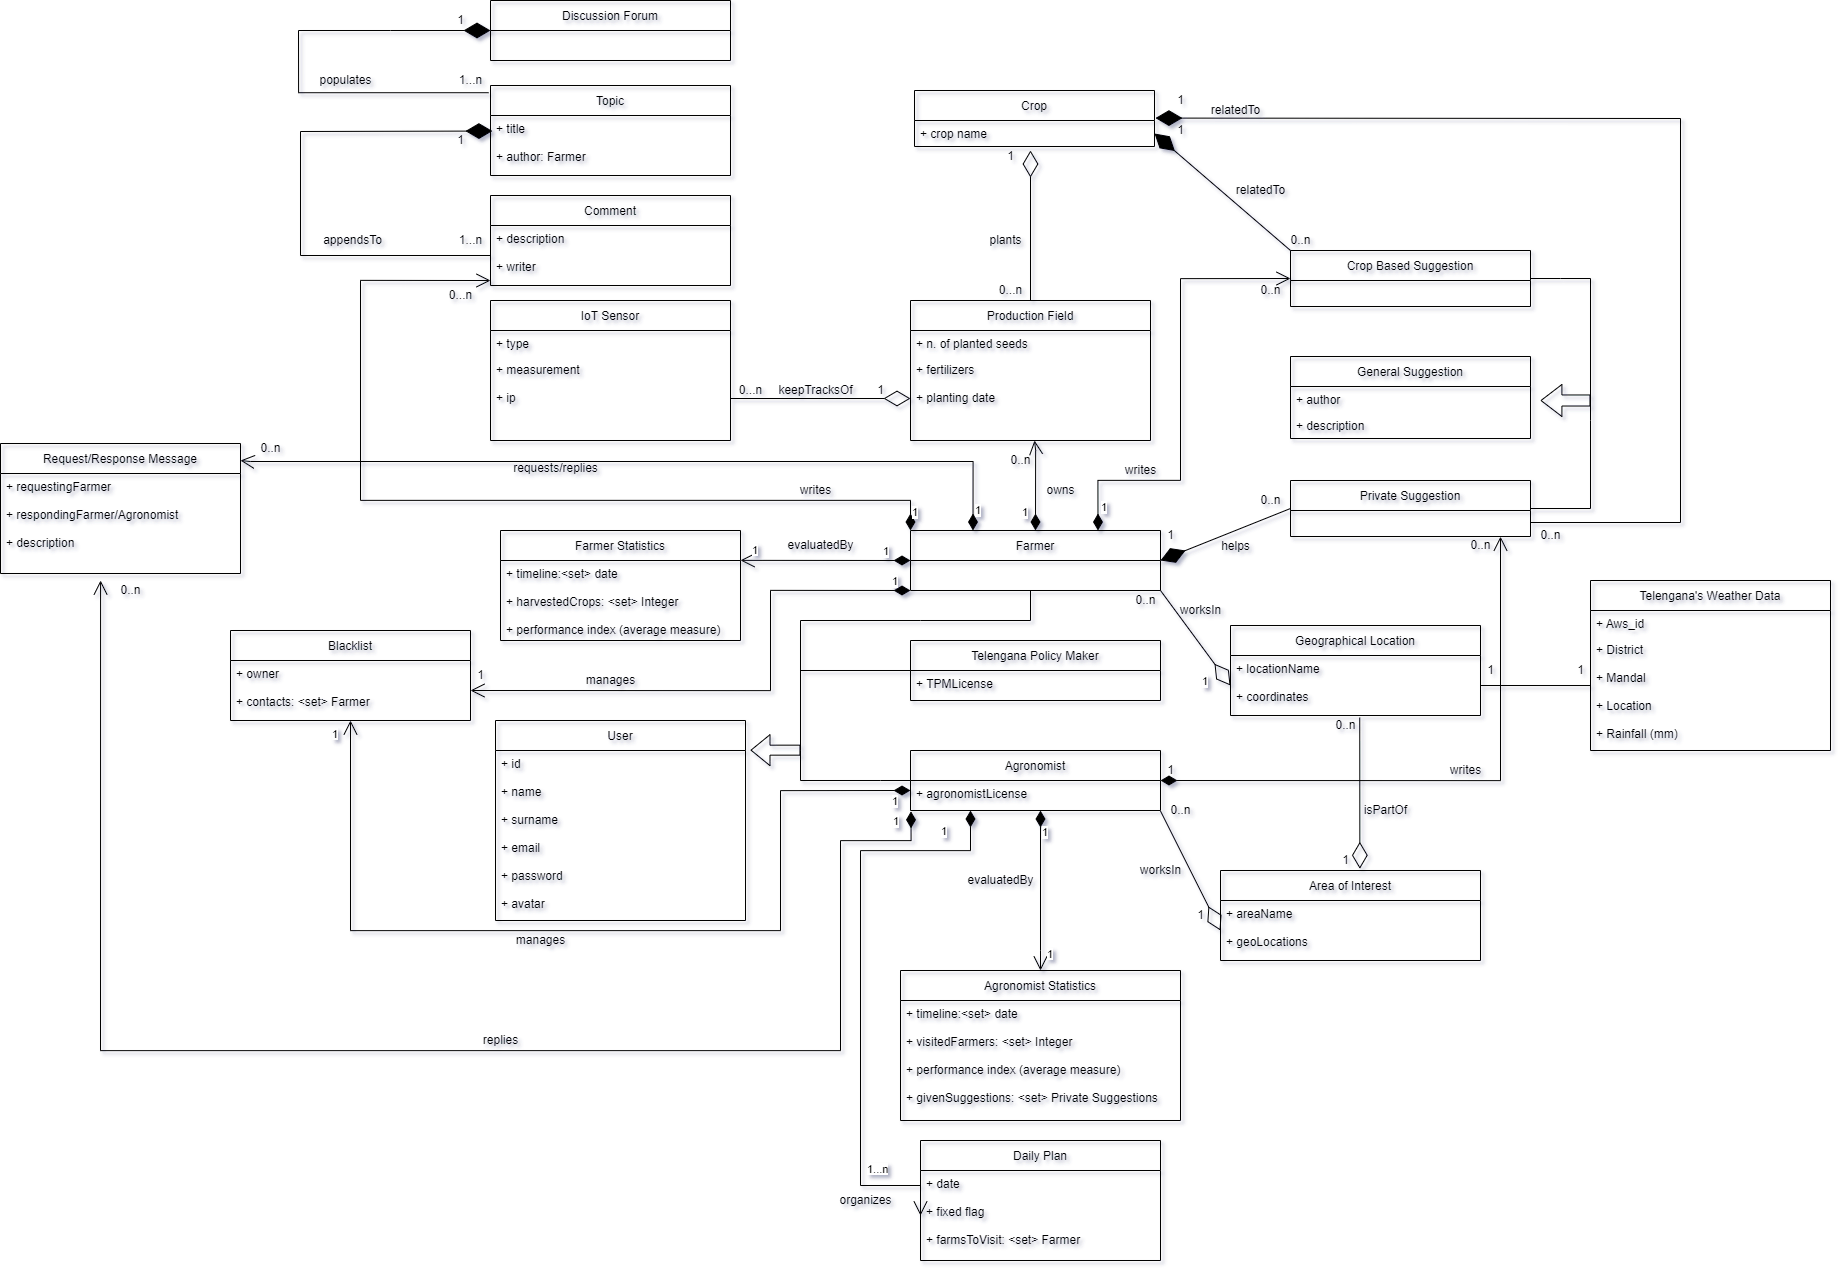
\includegraphics[width=\paperwidth - 1cm, angle=90]{/diagrams/classDiagramModel.png}
		\caption{\label{fig:classDiagram}High-level model structure}
	\end{figure}

	\FloatBarrier
	
	\subsubsection[State Diagrams]{\hyperlink{toc}{State Diagrams}}
	\label{sec:stateDiagrams}
		Considering now the main functionalities of the system, it is important to highlight the events that make its objects change their state. State diagrams are used to describe the most critical aspects of the objects previously described in the UML class diagram and how the systems manages them (\blueAutoref{fig:classDiagram}).
		
		\paragraph{Data Production Field}
			At the beginning the farmer compiles a form where he inserts the type of production (i.e the crop), the amount planted, the fertilizer, the date and the possible Iot devices associated. This event defines the beginning of a new production, so the system receives the data in the \textit{unprocessed} state, then it checks the correctness of the fields filled and at the end they are \textit{stored} in the data base. Here, the farmer can do different actions like doing \textit{updates} periodically inserting a comment, photo and a date. Also the \textit{IoT devices} declared weekly sends their data to the system and then stored in the database. At the end of a production cycle for the crops specified, the farmer inserts the ultimate data production, so \textit{the amount effectively produced}. The system computes the \textit{index performance index} as the ratio between amount produced and planted. It stores the index in the database as \textit{statistics} and the diagram ends.
			
			\vspace{0.3cm}
			\begin{figure}[h]
				\centering
				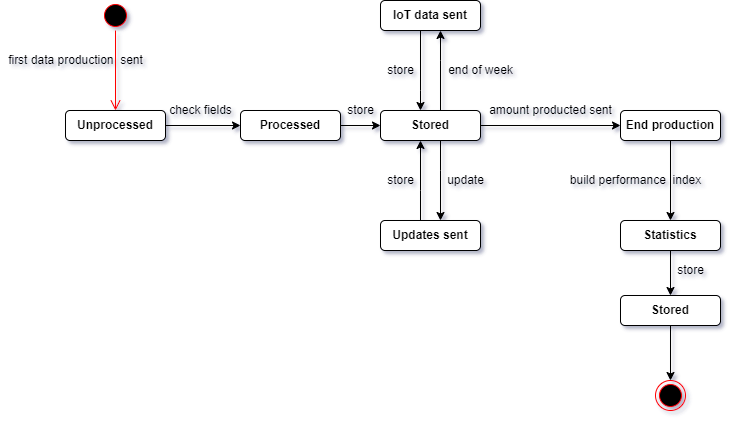
\includegraphics[scale=0.45]{/diagrams/state/dataproduction.png}
				\caption{\label{fig:dataproductionState}Data Production state diagram}
			\end{figure}
		
		\paragraph{Request}
			One of the main functionalities of the system is the intercation between farmers and agronomists through a direct \textit{request} for help. It is implemented like a chat window where it is possible to send messages, specifing the user selected and content of the message, and receive answers with little particular exceptions. In this situation the system search a farmer search an agronomist or another farmer and send \textit{request} data. The system doesn't send the request immediately to the possible receiver because it must check if he/she is present in a \textit{blacklist}. Every Agronomist and Farmer can block spammer users.
			If the check is completed succesfully, the request is \textit{stored} in the database, the system sends a \textit{notify} to the receiver \textit{marking it as un read}. 
			
			\vspace{0.3cm}
			\begin{figure}[h]
				\centering
				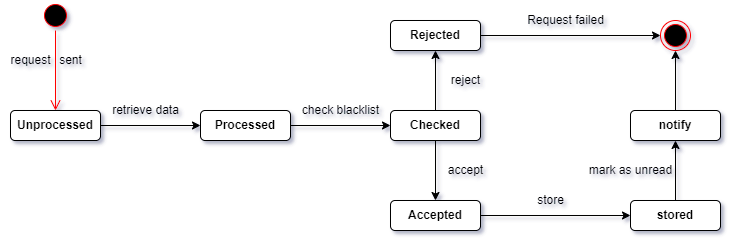
\includegraphics[scale=0.45]{/diagrams/state/request.png}
				\caption{\label{fig:requestState}Request state diagram}
			\end{figure}
		
		\paragraph{Forum}
			This state diagram emphasizes the forum functionality where farmers can interact surfing different topics and joining discussion. Each Farmer can publish a \textit{new topic} once per day to avoid spam, furthermore the system wants to discard off topic or recurring discussions. Every time a new topic is sent (where the title and the content is declared), the system checks the \textit{day limit} of the publisher, then it is \textit{accepted} and the topic is \textit{stored} in the database and visible to every users. Now we define a visible topic as \textit{regular}. Every user can report a topic, then the system checks the number of \textit{report} reached, if it is overtaken, the system \textit{deletes} the topic, otherwise the topic is still regular and visible to the users. When a user wants to \textit{comment} a topic, the system inserts the answer it in the database. 
			
			\vspace{0.3cm}
			\begin{figure}[h]
				\centering
				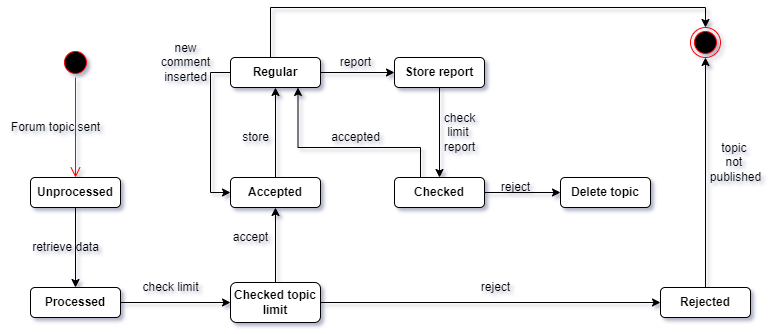
\includegraphics[scale=0.45]{/diagrams/state/forum.png}
				\caption{\label{fig:forumState}Forum state diagram}
			\end{figure}
		
		\paragraph{Daily Plan}
		This state diagram emphasizes the \textit{daily plan} functionality that describes how the agronomist's daily plan is managed. At the beginning of a \textit{new day} the system shows the \textit{new empty daily plan} tab for each agronomist. Now the user can modify the daily plan as he wants, he \textit{adds visits} and then he can \textit{update} the plan \textit{deleting} some existing ones or adding other visits. The page displays the \textit{confirm} button and only when the agronomist ends, so he has definitively decided which farm he must visit or he just visited, the user confirm the completation of the plan and it cannot be modified anymore and stored in the database. If a plan of a certain day is not confirmed, it will appear in the page in the future days, the user can modify past daily plans and confirm them. At the end of each month if some plans are not confirmed by the user, they will be confirmed definitely by the system. Each time a plan is confirmed, the visits to the farmers definied will be marked.
		
		\vspace{0.3cm}
		\begin{figure}[h]
			\centering
			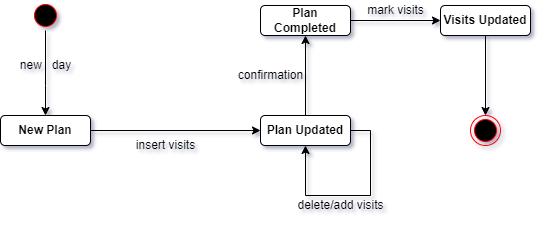
\includegraphics[scale=0.45]{/diagrams/state/dailyplan.png}
			\caption{\label{fig:dailyplanState}Daily Plan diagram}
		\end{figure}      

\subsection[Product Functions]{\hyperlink{toc}{Product Functions}}
	\label{sec:productFunctions}
	DREAM is an application that, on the one hand, provides a better cooperation between farmers, agronomists and TPMs, through direct requests or forums, as a social application, on the other hand the system monitors the development of the production through the computation of the statistics in order to improve the results. So one of the crucial function of the system is the collection of \textbf{data production}, and how the data are managed and visualized. Thanks to the geolocalization of the farmers and the assignment of the agronomists to a certain area is possible to simplify the visits to farms through the \textbf{daily plan} function. \textbf{Forum}, \textbf{request} and \textbf{personalized suggestions} functions are responsable for users interaction and knowledege exchange.\\
	
	Before starting with the description it is important to highlight that in order to benefit of DREAM functionalities the customer \textbf{must} be logged in the system as he can be recognized.
	
	\subsubsection[Data Production Field Function]{\hyperlink{toc}{Data Production Field Function}}
		\label{sec:dataproductionFunction}
		Farmers are allowed to insert data production thanks to DREAM: the managing process takes place entirely inside the application. It starts when the farmer plants a specified amount of a new crop and ends when the production is completed and it is known the amount of that crops has been produced. So in this way all coltivations cycle of a farm are well tracked constantly. Each farmer can also insert \textbf{updates} periodically through a text or photo about the status of the plants. Furthermore Iot devices send weekly data abount system irrigation and the humidity of the soil. This is usefull to keep Agronomists and Farmers up to date about the progession.  \\
		
		The data production functionality is provided to the user by an interface that allows him to insert all the information needed to store, manage and visualize data. The fields a user fills are reported here with a label that describes if they are mandatory or not.
		
		\begin{itemize}
			\item \textbf{Crop}\texttt{[MANDATORY]:} users must select a crop between a vaste selection. The system doesn't permit user to insert whatever text he or she wants to insert to avoid useless errors. This field is crucial to identify a specific coltivation and to receive in the future personalized suggestions for the crop inserted. It is possible to insert the same crop of an existing coltivation because maybe it has been planted in another moment or in different way. 
			
			\item \textbf{Amount}\texttt{[MANDATORY]:} this numerical field is marked as mandatory because, as we have previously said, the system manages the data to build statistics, so this is essential to compute the build performance index of that specific coltivation for that farmer. Obviously this input must be well managed and checked because no negative values are accepted.
			
			\item \textbf{Fertilizer}\texttt{[OPTIONAL]:} users need to give additional information providing also the type of the fertilizer to add more information on the method of the cultivation. It is not mandatory because it may be possible to avoid using fertilizer.
			
			\item \textbf{Date}\texttt{[MANDATORY]:} user must insert the start date of the production, this date must be equal to that of the planting date. The system doesn't fill this field automatically providing the users to add the new data production field whenever he wants.
			
			\item \textbf{IoT sensors}\texttt{[OPTIONAL]:} users should be able to monitor the humidity of the soil or the irrigation system through Iot sensors which, if they are available, send their values weekly directly to DREAM in order to \textbf{update} the status of the cultivation. This field must be filled with the IP address of the IoT devices.
		\end{itemize}
	
	All these fields are crucial to initialize a new data production field cycle and monitor it. Once all these data are sent and stored to the database, they are visible on the farmer data page to give also usefull information to agronomists to know how the farmer is working. Only the agronomists of the area which the farmer belongs, can visualize these data. \textit{Crop} is used to retrieve all the suggestions released about the crop specified. \textit{Amount} is a value used during the phase of end production to compute the performance index related only to that production cycle. The performance index is built on the dependencies of amunt planted, amount harvested and weather forecasts (e.g rainfall value).  
		

	\subsubsection[Request Function]{\hyperlink{toc}{Request Function}}
		\label{sec:requestFunction}
	The \textit{Request function} is used to create an interaction between Farmers and Agronomists, but in particular the idea is that to give the possibility to Farmers for \textit{solving problems} or asking curiosities directly to someone more competent in a specific field. Before sending the request through a \textit{message}, the system allows Farmers to \textit{search} whoever he wants and select the Farmer or the Agronomist he wants to get in touch with. So the Farmer can search another known and competent Farmer or maybe the Agronomist of its specific area. He must know the name and the surname of the user. When the user has been select, a new window appears and a field must be filled:
		 
		\begin{itemize}
			\item \textbf{Description}\texttt{[MANDATORY]:} This is a text area where the Farmer inserts the problem or whatever he wants to ask to the receiver. The field must not be empty, otherwise the message is not be sent. 
		\end{itemize}
	
	After the request has been sent, the addressee will receive a new \textit{notification} and the new request appears in the home page. The receiver (e.g Farmer, Agronomist) can check the requests, read the message and reply thorugh the same method. Farmer and Agronomist in their \textit{home page} visualizes all the requests received and sent. The request function is nt available for that users inserted in the \textbf{blacklist}
	
	\subsubsection[Forum Function]{\hyperlink{toc}{Forum Function}}
		\label{sec:forumFunction}
	Farmers usually don't get in touch in the real life because of the distance, working solitary in the farms. It is crucial an horizontally sharing of knowledge especially who plants the same cultivations or who deals with the same climate and soil conditions for example. The system shares a space dedicated only for Farmer through the Forum function. Each Farmer can enter the Forum visualizing topics and comments related to them, creating a new Topic, or partecipating to an existing topic through new comments. In this way DREAM connects all the Farmers registrated to the platform. When the Farmer adds a new topic must fill some fields:
	
		\begin{itemize}
	 		\item \textbf{Title}\texttt{[MANDATORY]:} This field is a text area and it usefull to identify briefly the topic discussion and what is inserted appears in the list of topics available in the forum home page.
	 		
	 		\item \textbf{Question}\texttt{[MANDATORY]:} When a new topic has been created, the discussion has to start with a question point, something that attracts answers and new comments in order to create a comparison. This field is a text area.
		\end{itemize}
	
	Every time a Farmer selects a topic, he visualizes all the comments related and he can add a new comment with a simple text area. After this, the new comment is visualized by all farmers. All topics or comments that are not ineherent will be reported by the users, so at a certain point, when the limit number of reportation has been reached, the system deletes them.
	This is important to avoid spam and delete useless topics.
	
	\subsubsection[Daily Plan Function]{\hyperlink{toc}{Daily Plan Function}}
		\label{sec:dailyplanFunction}
	Agronomists have to monitor the progession of the farmers' production, helping them with appropiate suggestions, answering their requests and especially visiting them directly in their farms. The agronomist must visits all of the farmers of their area of interest at least twice a year. The daily plan function keeps track of the visits for each agronomist, organizing in an appropriate manner agronomist daily work. Every day a new daily plan is published in the home page of the agronomist where he can interact with, managing, adding or deleting appointments. When the agronomist add an appointment, he must fill some fields:
		
		\begin{itemize}
			\item \textbf{Search}\texttt{[MANDATORY]:} The agronomist when add a new appointment, must declare the farmer that is visited. He searches through name and surname and he visualizes only farmers on its area of interest.
			
			\item \textbf{Note}\texttt{[OPTIONAL]:} This fields is a textarea that adds some information to the visit defined.It helps the agronomist to remember something in particular because it appears in the home page.
		\end{itemize}
		
	A daily plan can be confirmed whenever the agronomists want (also after some days), but in this way, the system do not allow agronomist to manage that daily plan for that day anymore. After the confirm, it will be stored and the system updates the visits. At the end of each month, every daily plan not confirmed, will be definitively stored by the system. The agronomist is notified when a farmer has not been visited.
	
	\subsubsection[Suggestion Function]{\hyperlink{toc}{Suggestion Function}}
		\label{sec:suggestionFunction} 
	The Agronomist can't interact directly with the farmers but he answers only to the request received, but now with the suggestion function is possible. Each statistic, update of the farmer can be seen and analyzed by the agronomist who is responsible of suggesting them correction, or best practies to improve their production, for example. This kind of suggestion is addressed only to farmer specified, so the system calls it \textbf{private suggestion}. When an agronomist wants to give a suggestion to a certain farmer, after he selects the option on the production field page of the farmer, he must fill some fields:
	
		\begin{itemize}
			\item \textbf{Crop}\texttt{[OPTIONAL]:} The agronomist must specify which crop the suggestion is related to. He can choose also to write the suggestion wthout specifying a crop.
			
			 \item \textbf{Description}\texttt{[MANDATORY]:} It is a text area where the agronomist describes the suggestion to give.
		\end{itemize}
	
	There exists another type of suggestion called \textbf{crop suggestion}. In this case, the suggestion is written by a farmer towards all the other farmers, but this is visualized in the production field of each farmer. In this situation the crop field is mandatory because the suggestion is visualized by all farmers who planted that specific crop.  
		
		
\subsection[User Characteristics]{\hyperlink{toc}{User Characteristics}}
	\label{sec:userCharacteristics}
	DREAM in Telangana has three different figure that are very important to distinguish in order to provide correctly the functionalities previously described in subsection \blueRef{sec:productFunctions}.
	
	\begin{itemize}
		\item \textbf{FARMER}
			\begin{itemize}
				\item Can register to the application.
				\item Always inserts correct data while registering.
				\item Can login in the application.
				\item Specify one and only one geographical area of working.
				\item Can insert in the system data about their production.
				\item Can insert updates related to a production field in the system.
				\item Can visualize data relevant (e.g build performance index, charts) to its production.
				\item Can access to the forum, reading all topics, adding new one or comment an existing one.
				\item Can retrieve suggestions from another Farmer or from an Agronomist.
			\end{itemize}
		\item \textbf{AGRONOMIST}
			\begin{itemize}
				\item Can register to the application.
				\item Always inserts correct data while registering and insert their vaild license.
				\item Can login in the application.
				\item Specifies at least one area of interest.
				\item Can visualize data concerning farmers that belong to its area of interest.
				\item Can visualize best and worst performing farmers.
				\item Can receive requests from a farmer. 
				\item Can include a farmer in a black list to avoid spam requests.
				\item Can send suggestions to the farmer.
				\item They have a daily plan about their visit to the farmer.
				\item Can update their daily plan.
				\item Can confirm a daily plan.
			\end{itemize}
		\item \textbf{TELANGANA'S POLICY MAKER}
			\begin{itemize}
				\item Can register to the application.
				\item Always inserts correct data while registering and insert their vaild license.
				\item Can login in the application.
				\item Can visualize farmers sorted by their performance.
				\item Identify those farmers who need to be helped.
				\item Can visualize Agronomist statistics. 
			\end{itemize}
	\end{itemize}
	
\subsection[Domain Assumptions]{\hyperlink{toc}{Domain Assumptions}}
	\label{sec:domainAssumptions}
	Domain assumptions are used to define clearly the world in which DREAM works. Thanks to them, we are able to add constraints that define the bounds of the environment. \\
	
	We assume that these assumptions hold true in the domain of the system:
		
	\begin{enumerate}[label=\textbf{DA\arabic*}]
		\item \label{dom:D1} Data concerning meteorological short-term and long-term forecasts are available from third party components. 	
		\item \label{dom:D2} Areas inserted by Agronomists and Farmers correspond to existing geographical locations.
		\item \label{dom:D3} Agronomists visit all farms at least twice a year.
		\item \label{dom:D4} Agronomists visit under-performing farms more than twice a year.
		\item \label{dom:D5} Information provided by the farmers about their work are coherent with their production.
		\item \label{dom:D6} Sensors devoted to obtain territory's measurement work and provide good approximations.
		\item \label{dom:D7} The water irrigation system works and provides correct measurements.
		\item \label{dom:D8} Farmer's request for help are well formulated and understandable.
		\item \label{dom:D9} Agronomists actually visited farms when they declare it in the daily plan.
		\item \label{dom:D10} Agronomist visits the same farms which has been declared in the daily plan.
		\item \label{dom:D11} The person who visits the related farm is verified to be the same agronomist declared in the system.
		\item \label{dom:D12} Suggestions related to production are well formulated, understandable and corenert with the corresponding request.
		\item \label{dom:D13} Suggestions related to production are actually coming from a competent farmer/agronomist.
		\item \label{dom:D14} Agronomists and Telengana's policy maker own a valid license.
		\item \label{dom:D15} Geographical area of interest are divided somehow equally among agronomists.
		\item \label{dom:D16} Each Farmer works only on a single location.
		\item \label{dom:D17} Sensors forwards error-free data through the communication network.
		\item \label{dom:D18} The farmers registered truly have a farm in the location specified.
		\item \label{dom:D19} Registered user are associated to existing and valid anagraphical identities.
		\item \label{dom:D20} IoT Irrigation system sensors send periodically and correctly data to the system about the amount of water used.
		\item \label{dom:D21} IoT territory sensors send periodically and correctly data about the measurement of the humidity of the soils.
		\item \label{dom:D22} Each photo and comment uploaded by the farmer is coherent with that specific crop published.
	\end{enumerate} 
	